\documentclass[a4paper,12pt]{article}
\usepackage[utf8]{inputenc}
\usepackage{cludein} 
\usepackage{xcolor}
\usepackage[toc,page]{appendix}
\usepackage{algorithm2e}
\usepackage{url}
\usepackage{hyperref}
\definecolor{light-gray}{gray}{0.5}
% Definindo novas cores
\definecolor{verde}{rgb}{0.25,0.5,0.35}
\definecolor{jpurple}{rgb}{0.5,0,0.35}
% Configurando layout para mostrar codigos Java
\usepackage{listings}
\DeclareGraphicsExtensions{.pdf,.png,.jpg}
\lstset{
  language=Java,
  basicstyle=\ttfamily\small, 
  keywordstyle=\color{jpurple}\bfseries,
  stringstyle=\color{red},
  commentstyle=\color{verde},
  morecomment=[s][\color{blue}]{/**}{*/},
  extendedchars=true, 
  showspaces=false, 
  showstringspaces=false, 
  numbers=left,
  numberstyle=\tiny,
  breaklines=true, 
  backgroundcolor=\color{cyan!10}, 
  breakautoindent=true, 
  captionpos=b,
  xleftmargin=0pt,
  tabsize=4
}
\pagestyle{plain}
\pagenumbering{arabic}
\usepackage[portuguese]{babel}
\addto\captionsportuguese{
\renewcommand{\figurename}{Fig.}
\renewcommand{\tablename}{Tab.}}
\begin{document}
\title{Relatório de Implementação dos Algoritmos}
\author{Heron Sanches \and Marino Honenheim \and Nilton Vasques\\\\
	Disciplina Teoria dos Grafos,\\
	Professor Steffen Lewitzka,\\
	Ciência da Computação,\\
	Universidade Federal da Bahia}
\date{\today}
\maketitle

\SetAlgorithmName{Algoritmo}{Lista de Algoritmos}

\section{Árvore Geradora Mínima}
Definição: Seja G=(V,E) um grafo não direcionado e conexo, G'=(V,E') é chamado de subgrafo gerador se possuí os mesmos vértices de G. Portanto se tivermos em G' uma árvore, então o subgrafo é uma árvore geradora. 
Quando G é um grafo conexo, em que cada aresta possui um valor ou peso p(e), o peso total da árvore geradora é \[\sum_{e \in E'}p(e)\] onde p(e) é uma função que retorna o peso da aresta \emph{e}. Á árvore geradora mínima é a árvore G' que possui o menor peso total dentre todas as árvores possíveis do grafo G\cite{nogueira}. Podemos enunciar a função para encontrar a árvore geradora mínima como \[\emph{min}\sum_{e\in E'}p(e)\].
A partir dessa noção podemos visualizar que encontrar a árvore geradora mínima não é tão trivial assim. Se propormos uma solução pela força bruta, ou seja, encontrar todas as árvores geradoras e assim então verificar qual a que possui o menor peso total. No pior caso quando temos um grafo completo(em que todos os vértices se ligam uns aos outros) teríamos $n^{n-2}$ árvores geradoras onde n é o número de nós, sendo assim teríamos uma solução em tempo exponencial $O(n^n)$ e inviável \cite{unicamp}.
Diante deste cenário alguns matemáticos elaboram soluções para o problema das Árvores Geradoras Mínimas, se utilizando de heurísticas gulosas para encontrar a solução ótima. No presente artigo abordaremos o Algoritmo de Kruskal e o de Prim, como estudo de caso.

\subsection{Projeto}
A implementação dos algoritmos referente a árvore geradora mínima, consistiu no desenvolvimento de um applet para java, que facilitasse a visualização das etapas realizadas pelos algoritmos de Kruskal e Prim, de maneira bastante interativa. Todo o material produzido na implementação esta disponível em \cite{niltonvasques}.

\subsection{Algoritmo de Kruskal}
O algoritmo de Kruskal é um algoritmo guloso, que tem por objetivo encontrar uma árvore geradora mínima para um grafo conexo e valorado ( com pesos nas arestas ). Vale ressaltar que para árvores não conexas, o algoritmo encontra floresta geradora mínima, ou seja uma árvore geradora mínima para cada componente conexo do grafo. O algoritmo pode ser enunciado nos seguintes passos:

\begin{algorithm}[H]
\SetAlgoLined
\KwData{ Um grafo Conexo }
\KwResult{ Uma árvore geradora mínima a partir de um grafo conexo }
Criar uma floresta \emph{F}, onde cada vértice do grafo é uma árvore separada\;
Criar um conjunto \emph{S} contendo todos as arestas do grafo\;
\While { \emph{S} é não vazio}{
	Remova um aresta \emph{e} com peso mínimo de S\;
	Se \emph{e} conecta duas diferentes árvores, então adicione \emph{e} para floresta \emph{F}\;
	Caso contrário, discarte \emph{e}, ou seja se a escolha de \emph{e} gera um circuito em \emph{F}, discarte-a\;
}
\caption{Pseudo Código do algoritmo de Kruskal}
\end{algorithm}

\subsubsection{Implementação}
A implementação foi realizada em Java com uso da estrutura de dados de listas encadeadas para manipular os conjuntos disjuntos. O código fonte está disponível no Apêndice A. A seguir o pseudo código da implementação com as manipulações representadas pelas operações Union-Find :\\
\begin{algorithm}[H]
\LinesNumbered
\SetAlgoLined
\KwData{ V, E}
\KwResult{ A, W}
W $\gets$ 0; A $\gets$ vazio\;
\For{ $v \in V $ }{
	$ a[v] \gets\textbf{{\color{blue}make-set}(v)}$\;
}
$L \gets \textbf{ordene}(E ,w )$\;
$k \gets 0$\;
	\While{ $k \neq \mid V\mid-1$ }{
	\textbf{remove}(L, (u, v ))\;
	a[u] $\gets$ \textbf{{\color{blue}find-set}(u)}\; 
	a[v] $\gets$ \textbf{{\color{blue}find-set}(v)}\;
	\If{ $a[u] \neq a[v]$ }{
		$aceita (u,v)$\;
		$A \gets A \cup \{(u, v )\}$\;
		$W \gets W + w (u, v )$\;
		$k \gets k + 1$\;
	}
	$\textbf{{\color{blue}union}}(a[u], a[v])$\;
}
$\textbf{retorne} (A, W)$\;
\caption{Pseudo Código do algoritmo de Kruskal com UnionFind}
\label{kruskal}
\end{algorithm}

\subsubsection{Análise de Complexidade}
A estrutura de dados UnionFind mantém um conjunto de elementos particionados em vários subconjuntos não sobrepostos. O algoritmo que controla essa estrutura possui duas operações principais:
\begin{itemize}
\item Find: Determina de qual subconjunto um elemento pertence.
\item Union: Faz a união de dois subconjuntos em um só subconjunto.
\end{itemize}

A ordenação na linha 5 do algoritmo \ref{kruskal}, tem complexidade \emph{ $O( \mid E\mid log \mid E\mid )$ } e domina a complexidade das demais operações.
A repetição das linhas 7-17 será executado \emph{$O(\mid E\mid)$} no pior caso.
Logo, a complexidade total das linhas 9-10 será \emph{$O(\mid E\mid f(\mid V\mid))$}, onde $f(\mid V\mid))$ é complexidade da função \textbf{{\color{blue}find-set}}.
As linhas de 12 a 15 serão executados $\mid V\mid -1$ vezes no total, pois para um grafo contendo N vértices, precisamos de apenas N-1 arestas para interligar todos os nós e gerar uma árvore geradora mínima. 
Assim, a complexidade total de execução destas linhas será \emph{ $O(\mid V\mid . g(\mid V\mid)$} onde $g(\mid V\mid)$ é a complexidade de realizar \textbf{{\color{blue}union}}.
A complexidade do algoritmo de Kruskal será então: \[ \emph{ $O(\mid E\mid log \mid E\mid + \mid E\mid .f(\mid V\mid) + \mid V\mid . g(\mid V\mid)) $}\]
A estrutura de dados UnionFind foi implementada na sua forma simples, com o uso de uma lista encadeada. Sendo assim a complexidade da função find é \emph{$\omega(n)$}, e union tem complexidade \emph{$O(n)$} \cite{Cormem}. A complexidade final da implementação foi:
\[ \emph{ $O(\mid E\mid log \mid E\mid + \mid E\mid .\Omega(\mid V\mid) + \mid V\mid . O(\mid V\mid)) $}\]

A complexidade pode ser reduzida utilizando de uma estrutura de dados mais refinada para implementar a manipulação dos conjuntos disjuntos, como por exemplo usar uma lista encadeada e \emph{weighted-union heuristic}\cite{Cormem}, consegue-se uma complexidade de \emph{$O(m+nlogn) $} para realizar as \emph{m} operações de \textbf{{\color{blue}make-set}}, \textbf{{\color{blue}find-set}} e \textbf{{\color{blue}union}} \cite{Cormem}.
\newpage
\subsection{Algoritmo de Prim}
Assim como o algoritmo de Kruskal's o algoritmo de Prim utilizada também uma heurística gulosa para solucinar o problema da Àrvore Geradora Mínima. A heurística utilizada é procurar o caminho mais curto, dentre todos os possíveis, de maneira similar ao algoritmo de Djikstra. O algoritmo de Prim's tem uma propriedade de que as arestas em \emph{A} sempre forma uma árvore simples \emph{Fig.1}.

\begin{figure}[h!]
	\caption{Ilustração do Algoritmo de Prim}
	\centering
	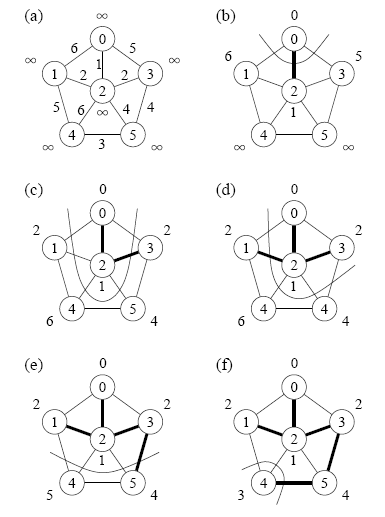
\includegraphics[width=0.5\textwidth]{prim}
	\label{fig:prim_fig}
\end{figure}

O algoritmo genérico de Prim procura encontrar o caminho mais curto de um vértice para os vértices vizinhos, até que todos os vértices estejão ligados uns aos outros. O pseudo-código pode ser visualizado logo abaixo:

\begin{algorithm}[H]
\SetAlgoLined
\KwData{ Um grafo Conexo }
\KwResult{ Uma árvore geradora mínima a partir de um grafo conexo }
Escolha um vértice S para iniciar o subgrafo\;
\While { há vértices que não estão no subgrafo }{
	selecione uma aresta segura\;
	insira a aresta segura e seu vértice no subgrafo\;
}
\caption{Pseudo Código do algoritmo de Prim}
\end{algorithm}

\subsubsection{Implementação}
Assim como a implementação anterior o algoritmo de Prim's foi implementado em Java e fez uso da Matriz de Adjacências Binária como estrutura de dados para armazenar os vértices adjacentes de um dado vértice u.  O código fonte está disponível no Apêndice A. O pseudo código que foi utilizado para a implementação pode ser visualizado em \emph{Algorithm 4}.

\begin{algorithm}[H]
\LinesNumbered
\SetAlgoLined
\KwData{ V, E}
\KwResult{ A, W}
dist[r] $\gets$ 0;
Q $\gets$ V\;
\For{ $v \in V-\{r\} $ }{
	$ dist[r] \gets \infty $\;
}
$ pred[r] \gets NULL$\;
$ A \gets \emptyset$\;
$ W \gets 0$\;
\While{  Q não for vazio  }{
	remover de Q o vértice u com menor valor em dist\;
	$ W \gets W + dist[u] $\;
	\If{ $ pred[u] \neq null $ } {
		$ A \gets A \cup \{(pred[u],u\}$\;
	}
	\For{ $ v \in Adj[u] $ }{
		\If{$v \in Q$ and $dist[v] > w[u,v] $} {
			$ dist[v] \gets w[u,v] $\;
			$ pred[v] \gets u $\;
		}
	}
}
$\textbf{retorne} (A, W)$\;
\caption{Pseudo Código do algoritmo de Prim}
\end{algorithm}

\subsubsection{Ánalise de Complexidade}

A complexidade do algoritmo de Prim está diretamente ligada a maneira de como é implementada a estrutura de dados em Q. Uma simples implementação utilizando matrizes de adjacência vai requerer complexidade \emph{$O(\mid V\mid^2)$} e foi a estrutura de dados utilizada neste trabalho. Utilizando de uma heap binária a complexidade cai para \emph{$O(\mid E\mid log\mid V\mid)$}, ainda assim é possível decrescer ainda mais a complexidade utilizando como estrutura de dados uma Fibonacci Heap com complexidade \emph{$O(\mid E\mid+\mid V\mid log\mid V\mid)$} \cite{Cormem}.


\section{Caminho Mínimo em Grafos Orientados}

\subsection{Algoritmo de Djikstra}
O algoritmo de Dijkstra, proposto pelo cientista E. W. Dijkstra, resolve o problema de encontrar o menor caminho entre dois vertices num grafo orientado ou não com arestas de peso não negativo.
O algoritimo de Dijkstra é um metodo guloso para resolver o problema do caminho mais curto.
A ideia por trás do método guloso é efetuar uma BFS ponderada sobre um dado grafo, a partir de um nó n. Dijkstra é comumente implementado com uma fila de prioridade como uma heap, de modo que em cada iteração, quando precisamos de obter o próximo nó a ser visitado, então este nó escolhido será o nó mais próximo ao nó n.

O algoritmo de Dijkstra mantem um conjunto S de vertices cujo o peso do menor caminho a partir de s já foi determinado. O algoritmo seleciona repetidamente o vértice $u \in V - S$ com o menor caminho estimado, acrescenta u em S, e relaxa todas as arestas que incidem em u. O seguinte pseudo-código usa uma fila de prioridade Q  de vértices, introduzidos pelos seus valores d.

\begin{algorithm}[H]
\LinesNumbered
\SetAlgoLined
\KwData{G,w,s}
INITIALIZE-SINGLE-SOURCE(G,s)\;
$ S \gets \emptyset $\;
$ Q \gets V[G] $\;
\While{ $Q = \emptyset $ }{
	$ u \gets EXTRACTING-MIN(Q) $\;
	$ S \gets S \cup \{u\} $\;
	\ForEach{ vertex $v \in Adj[u] $ }{
		RELAX(u,v,w)\;
	}

}
\caption{Pseudo Código do Algoritmo de Djijstra}
\end{algorithm}
\subsubsection{Análise de Complexidade}
Seja n o número de nós e m o número de arestas.

Uma vez que implementamos nossa fila de prioridade como uma heap, então o tempo de complexidade para remover o elemento minimo da heap ou adicionar um novo elemento é \emph{$O(log n)$}.
Agora precisamos considerar o fato de quando atualizamos as menores distância  dos nós, ou a fase de relaxação das arestas obtemos \emph{$O(n+m)$}.

Com isso, o tempo que o algoritmo de Dijkstra gasta em cada nó é \emph{$O(m log n)$}, enquanto que se precisamos visitar todos os nós, então a complexidade de tempo do algoritmo de Dijkstra seria \emph{$O((n+m)log n)$}.

Até agora, consideramos apenas a computação de um único nó para todos os outros nós. Contudo a complexidade para computar a menor distância partindo de todos os nós para todos os outros nós é \emph{$O(n (n+m)log n)$}. Assim, se temos um grafo completo a complexidade seria \emph{$O(n^2 log n)$}.

\subsubsection{Implementação}
O algoritmo foi implementado na linguagem python no arquivo dijkstra.py. Utiliza a biblioteca pygraphviz, que pode ser instalada em um computador Debian/Linux com o seguinte comando:

aptitude install python-pygraphviz

O arquivo dijkstra.py possui o seguinte cabeçalho:
\begin{lstlisting}
from pygraphviz import *
from random import *
from threading import Thread
import Image
import os
\end{lstlisting}

A função main contem os principais passos do algoritmo: 1) cria um grafo, os vértices e as arestas já são predefinidos; 2) exibe a imagem do grafo gerado; 3) cria uma matriz contendo os menores caminhos a partir de todos o vértices para todos os vértices; 4) solicita o vértice  origem e o vértice destino; 5) exibe a imagem do menor caminho de origem para destino.
\begin{lstlisting}
def main():

	# criao grafo
	grafo = criarGrafo() 
	grafo.draw("grafo.jpg", "jpg", "dot")
	#exibe o grafo
	Image.open("grafo.jpg").show();
	#calcula as distancias
	matriz = None
	matriz = calcularDistancias(grafo)
	//selecao dos vertices
	o = raw_input("\nEscolha um vertice de origem: ")
	#res = matriz.get(o)
	d = raw_input("Escolha um vertice destino: ")
	#desenha o menor caminho entre origem e destino
	desenharCaminho(grafo, matriz[o][1], o, d)
\end{lstlisting}
A função calcularDistancias irá executar o algoritmo de Dijkstra para todos os vértices como origem irá armazenar o resultado em uma matriz.
\begin{lstlisting}
def calcularDistancias(grafo):
	matriz = {}
	for v in grafo:
		dijk = Dijkstra()
		#calcula menor distancia de v para todos os outros vertices
		MenorDistancias = dijk.menorDistancias(grafo, v)
		; Armazena a  menor distancia partindo de v ate os outros vertices
		matriz[v] = MenorDistancias

	return matriz
\end{lstlisting}

O metodo menorDistancias da classe Dijkstra executa o algoritmo de dijkstra e retorna a lista dos menores caminhos do vertice v para os outros vertices.
\begin{lstlisting}
	def menorDistancias(self, grafo, v):

		#primeiro passo: iniciam-se os valores:
		distancia = {}
	
		for no in grafo:
			if no in grafo.neighbors(v): #se o no esta na lista dos vizinhos de v.
				distancia[no] = (float(grafo.get_edge(v, no).attr['label']), v) # armazena o peso da aresta
			else: # nao vizinho ou o mesmo vertice
				distancia[no] = (float('+inf'), None) # distancia = + infinito
	
		# Armazena a distancia partindo de v ate os outros vertices
		distancias = distancia.keys()
		vertices = [v]
		distanciaCopy = distancia.copy()
		listaDist = [distanciaCopy]

				
		while (len(distancias) > len(vertices)):
			ditems = distancia.items()
			daux = []
			for a in ditems:
				if a[0] not in vertices:
					daux += [a]

			menor = daux[0]
			for a in daux:
				if a[1][0]<menor[1][0]:
					menor = a

			vertices += [menor[0]]

			for no in grafo.neighbors(menor[0]):
				if no not in vertices:
					if distancia[no][0] > (menor[1][0]+float(grafo.get_edge(menor[0], no).attr['label'])):
						distancia[no] = (menor[1][0]+float(grafo.get_edge(menor[0], no).attr['label']), menor[0])

			
			distanciaCopy = distancia.copy()
			listaDist += [distanciaCopy]


		return (vertices, distancia, listaDist)
\end{lstlisting}
\newpage
\subsection{Algoritmo de Floyd-Warshall}
O algoritmo de Floyd-Warshall usa uma formulação de programação dinâmica para resolver o problema de caminhos mais curtos de todos os pares em grafo orientado G = (V,E). O algoritmo é executado no tempo \emph{$O(V^3)$}. 
O algoritmo de Floyd-Warshall se baseia na observação a seguir. Sejan V = {1,2,...,n} os vértices de G, e considere um subconjunto {1,2,...,k} de vertices  para algum k. Para qualquer par de vértices $i,j \in V$, considere todos os caminhos desde i até j cujos vértices intermediários são todos traçados a partir de {1,2,...,k}, e seja p um caminho de peso minimo dentre eles. O algoritmo de Floyd-Warshal explora um relacionamento entre o caminho p e caminhos mais curtos desde i até j com todos vértices intermediários no conjunto{1,2,...,k-1}. O Relacionamento depende do fato de k ser ou não um vértice intermediário do caminho p.

Se k não é um vértice intermediário do caminho p, então todos os vértices intermediários do caminho p estão no conjunto {1,2,...,k-1}. Desse modo, um caminho mais curto desde o vértice i até o j com todos os intermediários no conjunto {1,2,...,k-1} também é um caminho mais curto desde i até j com todos os vértices intermediários no conjunto {1,2,...,k}.

Se k é um vertice intermediário do caminho p, então desmembramos p em $ip_1kp_2j$. P1 é um caminho mais curto desde i até k com todos os vértices intermediários no conjunto {1,2,...,k}. Como o vértice k não é um vertice intermediário do caminho p1, vemos que p1 é um caminho mais curto desde i até k com todos os vértices intermediários no conjunto {1,2,...,k-1}. De modo semelhante, p2 é um caminho mais curto até o vértice j com todos os vértices intermediários no conjunto {1,2,...,k-1}.

\begin{figure}[h!]
	\centering
	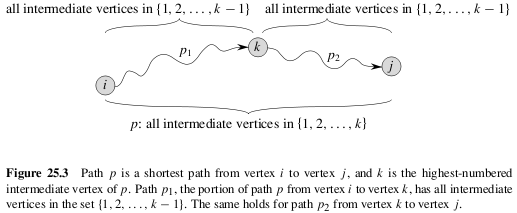
\includegraphics[width=1.0\textwidth]{djikstra}
	\label{fig:djikstra}
\end{figure}

A formulação recursiva seguindo a discussão acima é dada por:

\begin{figure}[h!]
	\centering
	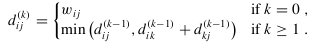
\includegraphics[width=0.5\textwidth]{djikstra2}
	\label{fig:djistra_pd}
\end{figure}

Com base na recorrência acima, o  seguinte procedimento bottom-up  pode ser usado para calcular o dij(k) , a fim de aumentar os valores de k. A sua entrada é uma matriz n x n W definido como na equação. O procedimento retorna a matriz D(n) com os pesos dos menores caminhos.

\begin{figure}[h!]
	\centering
	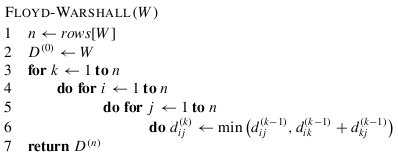
\includegraphics[width=0.8\textwidth]{floyd-warshall}
	\label{fig:floyd-warshall}
	\caption{Pseudo Código do algoritmo de Floyd-Warshall}
\end{figure}

\subsubsection{Implementação}
O algoritmo foi implementado na linguagem python no arquivo floyd.py.

A função main cria um grafo predefinido e depois chama a funcao floydWarshall com o gafo sendo passado como parâmetro.
\begin{lstlisting}
if __name__ == '__main__':
	
	#Cria o grafo

    grafo = {'A':{'A':0,'B':INF,'C':12,'D':6,'E':4},

             'B':{'A':INF,'B':0,'C':INF,'D':1,'E':INF},

             'C':{'A':INF,'B':INF,'C':0,'D':15,'E':3},

             'D':{'A':INF,'B':INF,'C':15,'D':0,'E':4},

             'E':{'A':INF,'B':7,'C':INF,'D':INF,'E':0}

             }
\end{lstlisting}
 
A funcão floydWarshall primeiro armazena a distancia dos vertices em seguida executa o algoritmo de Floyd-Warshal para obter o menor caminho para todos os pares por fim exibe a tabela com os resultados.
\begin{lstlisting}
def floydWarshall(grafo):

    nos = grafo.keys()

    distancia = {}
	
	#armezena a distancia do no n para o no k
    for n in nos:

        distancia[n] = {}

        for k in nos:

            distancia[n][k] = grafo[n][k]
	# Floyd-warshal - programacao dinamica
    for k in nos:

        for i in nos:

            for j in nos:

                if distancia[i][k] + distancia[k][j] < distancia[i][j]:

                    distancia[i][j] = distancia[i][k]+distancia[k][j]
	# imprime a tabela com resultado
    printSolution(distancia)
\end{lstlisting}

\newpage
\section{Busca em Profundidade ou Depth-First-Search (DFS) para Ordenação Topológica}

\subsection{Definição}
Busca em profundidade (ou busca em profundidade-primeiro, também usada a sigla em inglês DFS) é um algoritmo usado para realizar uma busca ou travessia numa árvore, estrutura de árvore ou grafo. Intuitivamente, o algoritmo começa num nó raiz (selecionando algum nó como sendo o raiz, no caso de um grafo) e explora tanto quanto possível cada um dos seus ramos, antes de retroceder(backtracking).

A estratégia seguida pela busca em profundidade é, procurar “mais fundo” no grafo sempre que possível. As arestas são exploradas a partir do vértice v mais recentemente descoberto que ainda tem arestas inexploradas saindo dele. Quando todas as arestas de v são exploradas, a busca “regressa” para explorar as arestas que deixam o vértice a partir do qual v foi descoberto. Esse processo continua até descobrirmos todos os vértices acessíveis a partir do vértice de origem inicial. Se restarem quaisquer vértices não descobertos, então um deles será selecionado como  nova origem, e a busca se repetirá a partir daquela origem. Esse processo inteiro será repetido até que todos os vértices sejam descobertos.

Sempre que um vértice v é descoberto durante uma varredura da lista de adjacências de um vértice já descoberto u, a busca em profundidade registra esse evento definindo um campo predecessor de v, um campo r[u], como u. O subgrafo predecessor produzido por uma busca em profundidade pode ser composto por várias árvores, ele forma uma floresta primeiro na profundidade composta por várias árvores primeiro na profundidade.
O algoritmo genérico para busca em profundidade realiza passos que já foram descritos mais acima. O pseudo-código pode ser visualizado no Algoritmo \ref{algorithm:buscaprofundidade}:\\ 
\begin{algorithm}[H]
\LinesNumbered
\SetAlgoLined
\KwData{ Inicio, Alvo }
function BuscaProfundidade\;{
  	empilha(Pilha,Inicio)\;
	\While { Pilha is not empty }{
		$var Nodo \gets desempilha(Pilha)$\;
	    	Colore(Nodo, Cinza)\;
	    	\If { Nodo = Alvo }{
	    		return Nodo\;
		}
	    	\For { Filho in Expande(Nodo)}{
      			\If {Filho.cor = Branco}{
        			empilha(Pilha, Filho)\;
			}
		}
    		Colore(Nodo, Preto)\;
		
	}
}
\caption{Pseudo-código do algoritmo de Busca em Profundidade}
\label{algorithm:buscaprofundidade}
\end{algorithm}

\subsection{Implementação}

A implementação deste algoritmo de busca em profundidade foi feito em C, fez uso de matriz de adjacências binárias como estrutura de dados para armazenar os vértices adjacentes de um dado vértice. O código fonte está disponível no Apêndice. O pseudo-código que foi utilizado para a implementação da busca em profundidade pode ser visualizado no Algoritmo \ref{algorithm:buscaprofundidade2}.

\begin{algorithm}[H]
\SetAlgoLined
\LinesNumbered
\KwData{Inicio, Alvo}
Coloque o nó inicial no topo da pilha\;
\If { pilha estiver vazia }{
	retorne falha e pare\;
}
\If{ o elemento na pilha é o nó alvo g}{
	retorne sucesso e pare\;
}\Else{
	Remova e expanda o primeiro elemebto e coloque o filho no topo da pilha\;
	Volte ao passo 2\;
}
\caption{Pseudo-código para a implementação de Busca em Profundidade}
\label{algorithm:buscaprofundidade2}
\end{algorithm}


\subsection{Análise de Complexidade}

O tempo de execução do nosso algoritmo de Busca em Profundidade é de tempo $O(V^2)$, para V igual à quantidade de vértices. Mas, a complexidade do problema pode ser de tempo O(V+E), sendo E a quantidade de arestas.
No nosso algoritmo, primeiro entra-se com um inteiro não negativo da quantidade de vértices do grafo, após isso diz-se qual o vértice-origem do grafo e o programa gera o vetor ordenado por Busca em Profundidade.

\subsection{Ordenação Topológica (usando Busca em Profundidade)}

Uma ordenação topológica de um grafo acíclico orientado G = (V,E) é uma ordenação linear de todos os seus vértices, tal que se G contém uma aresta (u,v), etnão u aparece antes de v na ordenação. A ordenação topológica de um grafo pode ser vista como uma ordenação de seus vértices ao longo de uma linha horizontal de tal forma que todas as arestas orientadas sigam da esquerda para a direita. 
Grafos acíclicos orientados (gao) são usados em muitas aplicações para indicar precedências entre eventos.\\


\begin{algorithm}[H]
\SetAlgoLined
TOPOLOGICAL-SORT(G)\;
chamar DepthFirstSearch (DFS) para cada vértice v\;
à medida que cada vértice é terminado, inserir o vértice à frente de uma lista ligada\;
return a lista ligada de vértices.\;
\caption{Pseudo Código para ordenar topologicamente um gao}
\end{algorithm}

\begin{verbatim}

\end{verbatim} 
Executamos uma ordem topológica no tempo O(V+E), pois a busca em profundidade demora o tempo O(V+E) e leva tempo O(1) para inserir cada um dos $\mid V\mid$ vértices à frente da lista ligada.

\begin{figure}[h!]
	\centering
	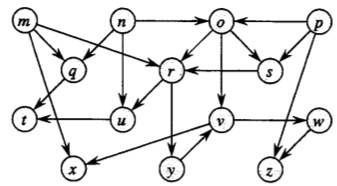
\includegraphics[width=0.6\textwidth]{gao}
	\label{fig:gao}
	\caption{Um gao para ordenação topológica}
\end{figure}

Para o exemplo a seguir, a matriz adjacência seria a que é mostrada na Fig 4.

\begin{figure}[h!]
	\centering
	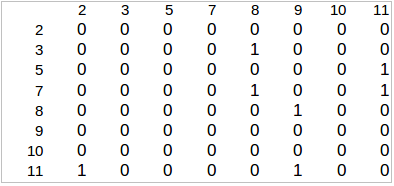
\includegraphics[width=0.6\textwidth]{matriz}
	\label{matriz}
	\caption{Matriz Adjacência para o grafo ao lado}
\end{figure}

\begin{figure}[h!]
	\centering
	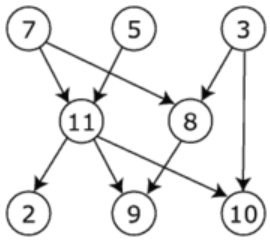
\includegraphics[width=0.4\textwidth]{grafodirecionado}
	\label{fig:grafodirecionado}
	\caption{Exemplo de grafo direcionado a ser ordenado por profundidade}
\end{figure}

Uma ordenação da busca profundidade para o exemplo seria $7 \to 11 \to 2 \to 9 \to 10 \to 5 \to 8 \to 3 \to 10$.
\newpage
\section{Fechamento Transitivo}

\subsection{Definição}
Suponha que temos um grafo direcionado G = (V,E). É útil saber que, dado um par de vértices u e w, onde há um caminho de u para w no grafo. Uma boa maneira de guardar esta informação é construir um outro grafo, chamá-lo de G* = (V, E*), tal que existe uma aresta (u, w) em G*, se e somente se, existe um caminho de u para w em G. Esse grafo é chamado de fechamento transitivo.

O nome “fechamento transitivo” significa que:
	Ter uma propriedade transitiva significa que se a se relaciona com b de alguma forma especial, e b se relaciona com c, então a se relaciona com c. Somos familiares com várias formas de transitividade. No caso de grafos, dizemos que um grafo é transitivo se, para todo trio de vértices a, b e c, se (a,b) é uma aresta, e (b,c) é uma aresta, então (a,c) também é uma ares. Alguns grafos são transitivos, outros não. Algebricamente: “R é transitiva sse $R^n \subseteq R$ para todo $n \geq 1$”. 
	Um conjunto A* é um fechamento de um conjunto A com alguma propriedade especial (como transitividade) é resultado da soma de A com somente os elementos que causam A satisfazer esta propriedade especial, e não outros elementos. O fechamento transitivo de um grafo é resultado da adição das menores arestas possíveis ao grafo tal que é transitivo. (Podemos facilmente adicionar uma porção de arestas a um grafo para fazê-lo transitivo, mas a parte do fechamento transitivo significa que queremos preservar as relações de caminhos existentes anteriormente, i.e., não adicionaremos arestas que não representam caminhos no grafo.
	Representaremos grafos usando uma matriz de adjacência de valores booleanos e usaremos esta matriz de adjacência para construir a matriz de fechamento transitivo. 

\subsection{Algoritmo de Warshall}
	
O algoritmo de Warshall é um algoritmo de força bruta, tem por objetivo encontrar para cada elemento do grafo, as arestas que chegam e saem dele. É um eficiente método de computar a transitividade de uma relação. O algoritmo de Warshall tem como entrada uma matriz Mr representando a relação R e tem como saída a matriz Mr* da relação R*, o fechamento transitivo de R. Abaixo está um pseudo-código para Warshall.

\begin{algorithm}[H]
Transitive-Closure (G)\;
        n = $\mid V\mid$\;
        t(0) = the adjacency matrix for G\;

        // there is always an empty path from a vertex to itself,
        // make sure the adjacency matrix reflects this

        \For{ i in 1..n }{
                t(0)[i,i] = True\;
        }

        // step through the t(k)'s\;

        \For{ k in 1..n }{
                \For{ i in 1..n}{
                        \For{ j in 1..n }{
                                $t^{(k)}[i,j] = t^{(k-1)}[i,j] OR (t^{(k-1)}[i,k] AND t^{(k-1)}[k,j])$\;
                        }
                }
        }
        return t(n)\;
	\caption{Pseudo-código do algoritmo de Warshall}
\end{algorithm}

\subsection{Implementação}

A implementação foi feita em Python. O código fonte está disponível no Apêndice. A seguir o pseudo código da implementação com a função principal do algoritmo de Warshall.

\begin{algorithm}[H]
\KwData{ MR: n x n 0-1 matrix }
$W := MR( W = [w_{i,j}] $)i
\For{k=1 to n }{
	\For{i=1 to n}{
		\For{ j=1 to n }{
			$w_{i,j} = w_{i,j} \vee ( w_{i,k} \wedge w_{k,j} )$\;
		}
	}
}
return W\;
\caption {Pseudo-código da função principal do algoritmo de Warshall}
\end{algorithm}


\subsection{Análise de Complexidade}

Ao final do algoritmo, a simples análise dele nos diz que a complexidade dos 3 loops levam um tempo $O(n^3)$. Com relação ao armazenamento de dados, notamos que no algoritmo só precisamos de duas matrizes computadas, então podemos reusar o armazenamento para outras matrizes, nos dando uma complexidade de armazenamento de $O(n^2)$.


\newpage
\appendix
\begin{appendices}

% When using section nested in appendices block, errors unexpected errors are happening
%\section{Algoritmos Implementados no Projeto} %\label{App:AppendixA}

\label{App:AppendixA}
\chapter{Algoritmos Implementados no Projeto}
 
\lstinputlisting[title=Implementação do Algoritmo de Kruskal em Java, language=Java, texcl=true]{Kruskal.java}
\lstinputlisting[title=Implementação do Algoritmo de Prims em Java, language=Java, texcl=true]{Prim.java}

\lstinputlisting[title=Implementação do Algoritmo de Djikstra em Python, language=Python, texcl=true]{dijkstra.py}
\lstinputlisting[title=Implementação do Algoritmo de Floyd em Python, language=Python, texcl=true]{floyd.py}

\lstinputlisting[title=Implementação do Algoritmo de Warshall em Python, language=Python, texcl=true]{warshall.py}
\lstinputlisting[title=Implementação da busca profundidade em C, language=C, texcl=true]{dfs.c}

%\section{Codigo Fonte das Estrutura de Dados Implementadas no Projeto} \label{App:AppendixE}

\chapter{Código Fonte das Estruturas de Dados Implementadas no Projeto}

\lstinputlisting[title=Interface Para Operações Union-Find com Lista Encadeada, language=Java, texcl=true]{UnionFind.java}
\lstinputlisting[title=Implementação da Matriz de Adjacências Binária, language=Java, texcl=true]{AdjacencyMatrix.java}

\end{appendices}

\bibliographystyle{plain}
\bibliography{biblio}

\end{document}


